\chapter{Proposed approach}
\label{chapter:proposedApproach}

For solving the problem of detecting malicious PDF documents, we came with a Machine Learning based approach. We took into account the importance of keeping the documents content confidentiality, as well as the need for ensuring the speed of analysis process. This solution will be next integrated into a Cloud framework responsible for remote documents scanning.

\section{Dataset}
\label{section:dataset}
The first step in building the optimal \textit{ML} model was to create a dataset which would train the classifier. Our target was to collect malicious and benign PDF samples used in real life scenarios. Circa 70\% of the clean and malicious documents were downloaded from the online malware repository \textit{Contagio} \cite{contagio}, which provides samples collected from various open sources. Nevertheless, for more recent malicious PDFs we used VirusTotal \cite{virustotal}, Hybrid Analysis \cite{hybridanalysis} and VirSCAN \cite{virscan}, that allow searching files by their hash (\textit{MD5}, \textit{SHA1}, \textit{SHA256}). Some of them provide access to the entire file collection so that we can order them by upload date and search for the most recent uploaded harmful files. Many clean samples were collected from public sources using Google Search Operators, i.e., \code{filetype:pdf}, for restricting search results of PDF files. Additionally, we completed the dataset with more than 100 clean interactive PDF files, that contain embedded 3D Widgets, incorporated JavaScript games etc. These clean samples should train the ML model, so as to correctly classify files even in corner cases. 

\begin{table}[H]
	\caption{Dataset of PDF samples}
	\label{table:pdfSamples}
        \centering
            \begin{tabular}{p{2.5cm} p{9.5cm}}
                \toprule
                
				\textbf{Category} & \textbf{Source} \\
				\hline 
                \texttt{benign} & Contagio, Google Queries, Tetra4D, PdfScripting \\
                \hline
				\texttt{malicious} & Contagio, VirusTotal, Hybrid Analysis, VirSCAN \\
                
                \bottomrule
			\end{tabular}
\end{table}

\section{Proof of Concept}
\label{section:poc}

In the following subsections we will touch upon algorithms and techniques we have used to achieve the purpose of this thesis, namely detecting malicious PDF documents using a Machine Learning based solution. Figure \ref{mlsteps} represents the entire process which was followed while developing the \textit{ML} model. Each process phase will be fathomed in the following.

\begin{figure}[H]
	\centerline{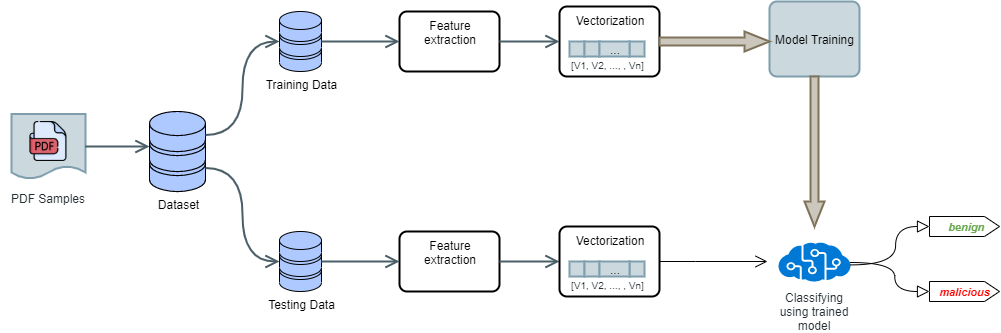
\includegraphics[scale=0.5]{figures/ml.png}}  
	\caption{Machine Learning model creation}
	\label{mlsteps}
\end{figure}

\subsection{Feature Selection}
As we already know, Machine Learning is based on mathematical concepts, hence the algorithms consist of performing mathematical operations to identify patterns in data. In order to use our dataset as input for ML algorithms, first of all we need to bring the data in an appropiate form. Therefor the most relevant data from a PDF document should be extracted and transformed into a vectorized form. As already seen in Table \ref{table:pdfentries}, there are several standard PDF entries which can be used for malicious intentions. For featurizing PDF documents we have used \textit{PDFiD} from \textit{PDF Tools} suite \cite{pdftools}, which is a Python script that selects 22 features from a PDF file, including keywords commonly found in malicious documents, name obfuscations etc. The output of the script is a list of PDF entries and their occurences (see Figure \ref{pdfidoutput}). Before turning this featurized form of the PDF file into input for ML algorithms, the data should be normalized to [0, 1] range. This is an important step in order to avoid ML issues when features are on drastically different scales (see \cite{mlCookbook}). The vectorized form of the PDF document is built by applying the \textit{Min-Max Normalization} (\ref{eq:1}) strategy on the array of features extracted by \textit{PDFiD}.

\begin{equation}
	\label{eq:1}
	z = \frac{x - min(x)}{max(x) - min(x)}
\end{equation}

\begin{figure}[H]
	\centerline{\includegraphics[scale=0.6]{figures/pdfidoutput.png}}  
	\caption{Example of results of \textit{PDFiD} applied on a benign PDF file (left) and on a malicious one (right)}
	\label{pdfidoutput}
\end{figure}

\subsection{Classification Techniques}
% p. 8 tsukermann book
\subsection{Performance Evaluation}
\subsection{Experiment}     % Metasploit + Kali
\cite{zeltser}

\section{Used technologies}
\label{section:technologies}
\subsection{Microsoft .NET Framework}
As previously mentioned in sections \ref{section:backgroundProc} and \ref{section:filesystem}, our application is going to have a help tool for Windows based computers that will automatically detect new downloaded PDF documents, upload them to our Cloud Analyzer and take action (keep/delete) on that files corresponding to their category (benign/malicious). This tool will take the form of a Windows Service which will start running at the boot-time of the computer in the Session 0 (see section \ref{section:backgroundProc}) and will communicate with an application responsible for notifying users through Windows notifications (see Figure \ref{winserviceDesign}). 

\begin{figure}[H]
	\centerline{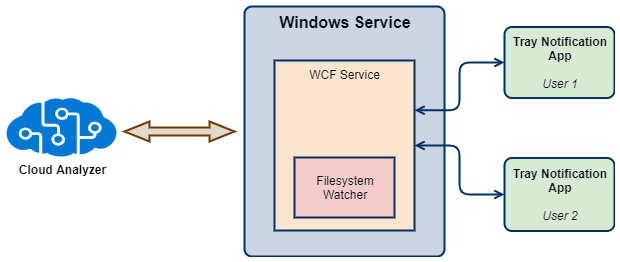
\includegraphics[scale=0.6]{figures/winService.png}}  
	\caption{Architecture's outline of the help tool for Windows}
	\label{winserviceDesign}
\end{figure}

Microsoft \textbf{.NET Framework} provides all the necessary Classes for creating the described tool. This framework represents a solution for standardization of application development on Windows operating system. Prior to the introduction of .NET Framework, the developers mostly used COMs\footnote{Component Objcet Model (COM) is a model of reusable software introduced by Microsoft in 1993} as a solution for code reuse. However, COM requires developers to write boilerplate code in order to turn their business logic into a reusable component, including memory clean up, reference counting etc, whence result a lot of errors. .NET Framework allow developers to focus on writing the business logic, while it is dealing with the memory management and is providing consistent exception-handling mechanisms. For example, in our application we implemented several .NET interfaces to achieve the expected behavior without having to manage a lot of low-level details. To create a Windows Service, we derived our class from \code{System.ServiceProcess.ServiceBase} and we had to override it's \code{OnStart}, \code{OnStop} methods. Because a service runs in Session 0, it means that it does not have support for user interface. Yet the application is intended to push Windows notifications and to ensure this functionality we had to treat our tool as a client-server application. The Windows service establishes an interprocess communication with the client \textit{Tray Notification App} when a user logs in. For this mechanism the WCF\footnote{Windows Communication Foundation (WCF) is a set an API in the .NET Framework for building connected, service-oriented applications} framework is integrated, which allows sending data as asynchronous messages from one endpoint to another. WCF was chosen as communication layer because it provides the \textit{duplex} message exchanging pattern, where two processes establish a secure TCP connection and can send data in both directions. To make this working, it is necessary to just define used entities for communication as \textit{Data Contracts}, that will later serialize the metadata by the WCF serialization engine. Another important component that lies at the core of the WCF service is the monitor class that inherits from .NET \code{System.IO.FileSystemWatcher}. It's behavior was described in section \ref{section:filesystem} and basically we use it to monitor user's specified folders and to send events to the users via the WCF communication. At the top level, in order to catch sent events from the Windows Service, a hidden WPF\footnote{Windows Presentation Foundation (WPF) is a UI framework for desktop applications from .NET Framework} application starts communication with the service at the user's login. When a PDF document is downloaded into monitored folder the Windows Service throws an event that is displayed to the user in form of a Windows System Tray Notification.

% Before putting to disposition of the user this tool, we had to create an installer (++ winService)

\subsection{Scikit-learn Machine Learning Library}
It would be extremely inefficient to always reimplement each Machine Learning algorithm that is required for solving a specific problem. \textbf{Scikit-learn} is one of the well known and largely used ML libraries, that came across as a solution for code reusability and performance optimization. This open-source library was created above the already prepared "ecosystem" for Data Science - \textit{Python}. Even Python is just a programming language, there are a plenty of created libraries using Python, that are used on a daily basis by scientists. In terms of efficiency there are no doubts, that Scikit-learn would give way to other ML libraries. And all this beacause of it's underlying technologies. At the core it integrates:
	\begin{itemize}
		\item \textit{Cython} - a compiled language that can bind compiled libraries, reaching high performance of the CPU;
		\item \textit{Numpy} - optimized Python module for working with large multidimensional arrays;
		\item \textit{Scipy} - a large collection of efficient algorithms for linear algebra, interpolation etc.
	\end{itemize}
Till now, the Scikit-learn developers have supplied the library with various supervised and unsupervised algorithms, such as: regression, clustering, classification algorithms, as well as: Random forest, Support Vector Machine etc. It is a perfect solution for both academic and commercial projects, because of the simple API that it provides, thus the generic implementation of the algorithms can be adapted to personal purposes.

\subsection{Python Flask}
\subsection{ReactJS Framework}
